% Commented out: 
% \addbibresource
% \includepdf

\documentclass[12pt,letterpaper,english,bibliography=totocnumbered, abstract=on]{scrartcl}

\usepackage{indentfirst}
\usepackage[titletoc]{appendix}
%\usepackage{fullpage}
%\usepackage{subfiles}
\usepackage[T1]{fontenc}
\usepackage[latin9]{inputenc}
\usepackage{color}
\usepackage{babel}
\usepackage{verbatim}
\usepackage[unicode=true,pdfusetitle,
bookmarks=true,bookmarksnumbered=false,bookmarksopen=false,
breaklinks=true,pdfborder={0 0 0},pdfborderstyle={},backref=false,colorlinks=true]
{hyperref}
\hypersetup{linkcolor=blue,citecolor=blue,urlcolor=blue}

\usepackage{booktabs}
\usepackage{multirow}
\usepackage{adjustbox}
\usepackage{threeparttable}
\usepackage[table]{xcolor}
\usepackage{csquotes}
\usepackage{soul} % for hiliting text: \hl

\usepackage[backend=biber, style=authoryear, maxbibnames=99, dashed=false]{biblatex}
\setlength\bibitemsep{2\itemsep}
\addbibresource{refs.bib}

\usepackage{pdfpages}
\usepackage{float} % Allows use of H to place floats

\usepackage{pgfgantt}

\usepackage{framed}

\usepackage{subcaption}

% Prevent page breaks within paragraphs
% https://tex.stackexchange.com/questions/21983/how-to-avoid-page-breaks-inside-paragraphs
\widowpenalties 1 10000

% The following package automatically provides ragged right formatting for text within table cells.
\usepackage[raggedrightboxes]{ragged2e}

\begin{document}

\titlehead{DRAFT}

\title{Proposed Method for Dosing Coconut Rhinoceros Beetle Adults with OrNV}

\author{Aubrey Moore and Laura Caser \\ University of Guam}

%\date{May 5, 2020\\Revised May 4, 2021}

\maketitle
%\footnote{\url{https://github.com/aubreymoore/2020-FS-CRB-biocontrol-project/blob/master/combined-proposal.pdf}}
%\newpage
%\tableofcontents

\pagebreak

\section{Introduction}

Several methods have been used to dose coconut rhinoceros beetle adults (CRB) with \textit{Oryctes rhinoceros} nudivirus (OrNV): 

\begin{table}[h]
	\centering
	\begin{tabular}{p{1.5in}p{1.5in}p{1.5in}}	
		\toprule
		Method & Pros & Cons \\
		\midrule	
		Application of droplets containing OrNV particles to mouthparts 
		& Requires very little OrNV 
		& Amount ingested may be highly variable \\
		\midrule
		Forcing CRB to swim in an aqueous suspension containing OrNV particles 
		&  
		& Requires a large amount of OrNV \\
		\midrule
		Direct injection into the hemocoel 
		& Unatural  
		& Allows for precise dosing. Requires a very small amount of OrNV. \\
		\bottomrule
	\end{tabular}
\end{table}

We propose an alternative dosing method which models feeding behavior of CRB adults within bore holes. A CRB adult usually initiates boring behind a petiole. The beetle typically bores horizontally into the center of the crown-shaft and then bores downwards. The beetle feeds on sap when exudes from tissue which is macerated during the boring activity.

In our dosing technique, we confine a beetle to the bottom of a disposable centrifuge tube (details) which models the vertical portion of a bore hole (Fig. \ref{fig:crb-in-tube}). Before introducing a beetle, 2 ml of 5\% sucrose solution containing 10\textsuperscript{6} infectious units of OrNV  are added to the tube. This liquid models sap from which collects at the bottom of the vertical section of a borehole.

% TODO: \usepackage{graphicx} required
\begin{figure}[H]
	\centering
	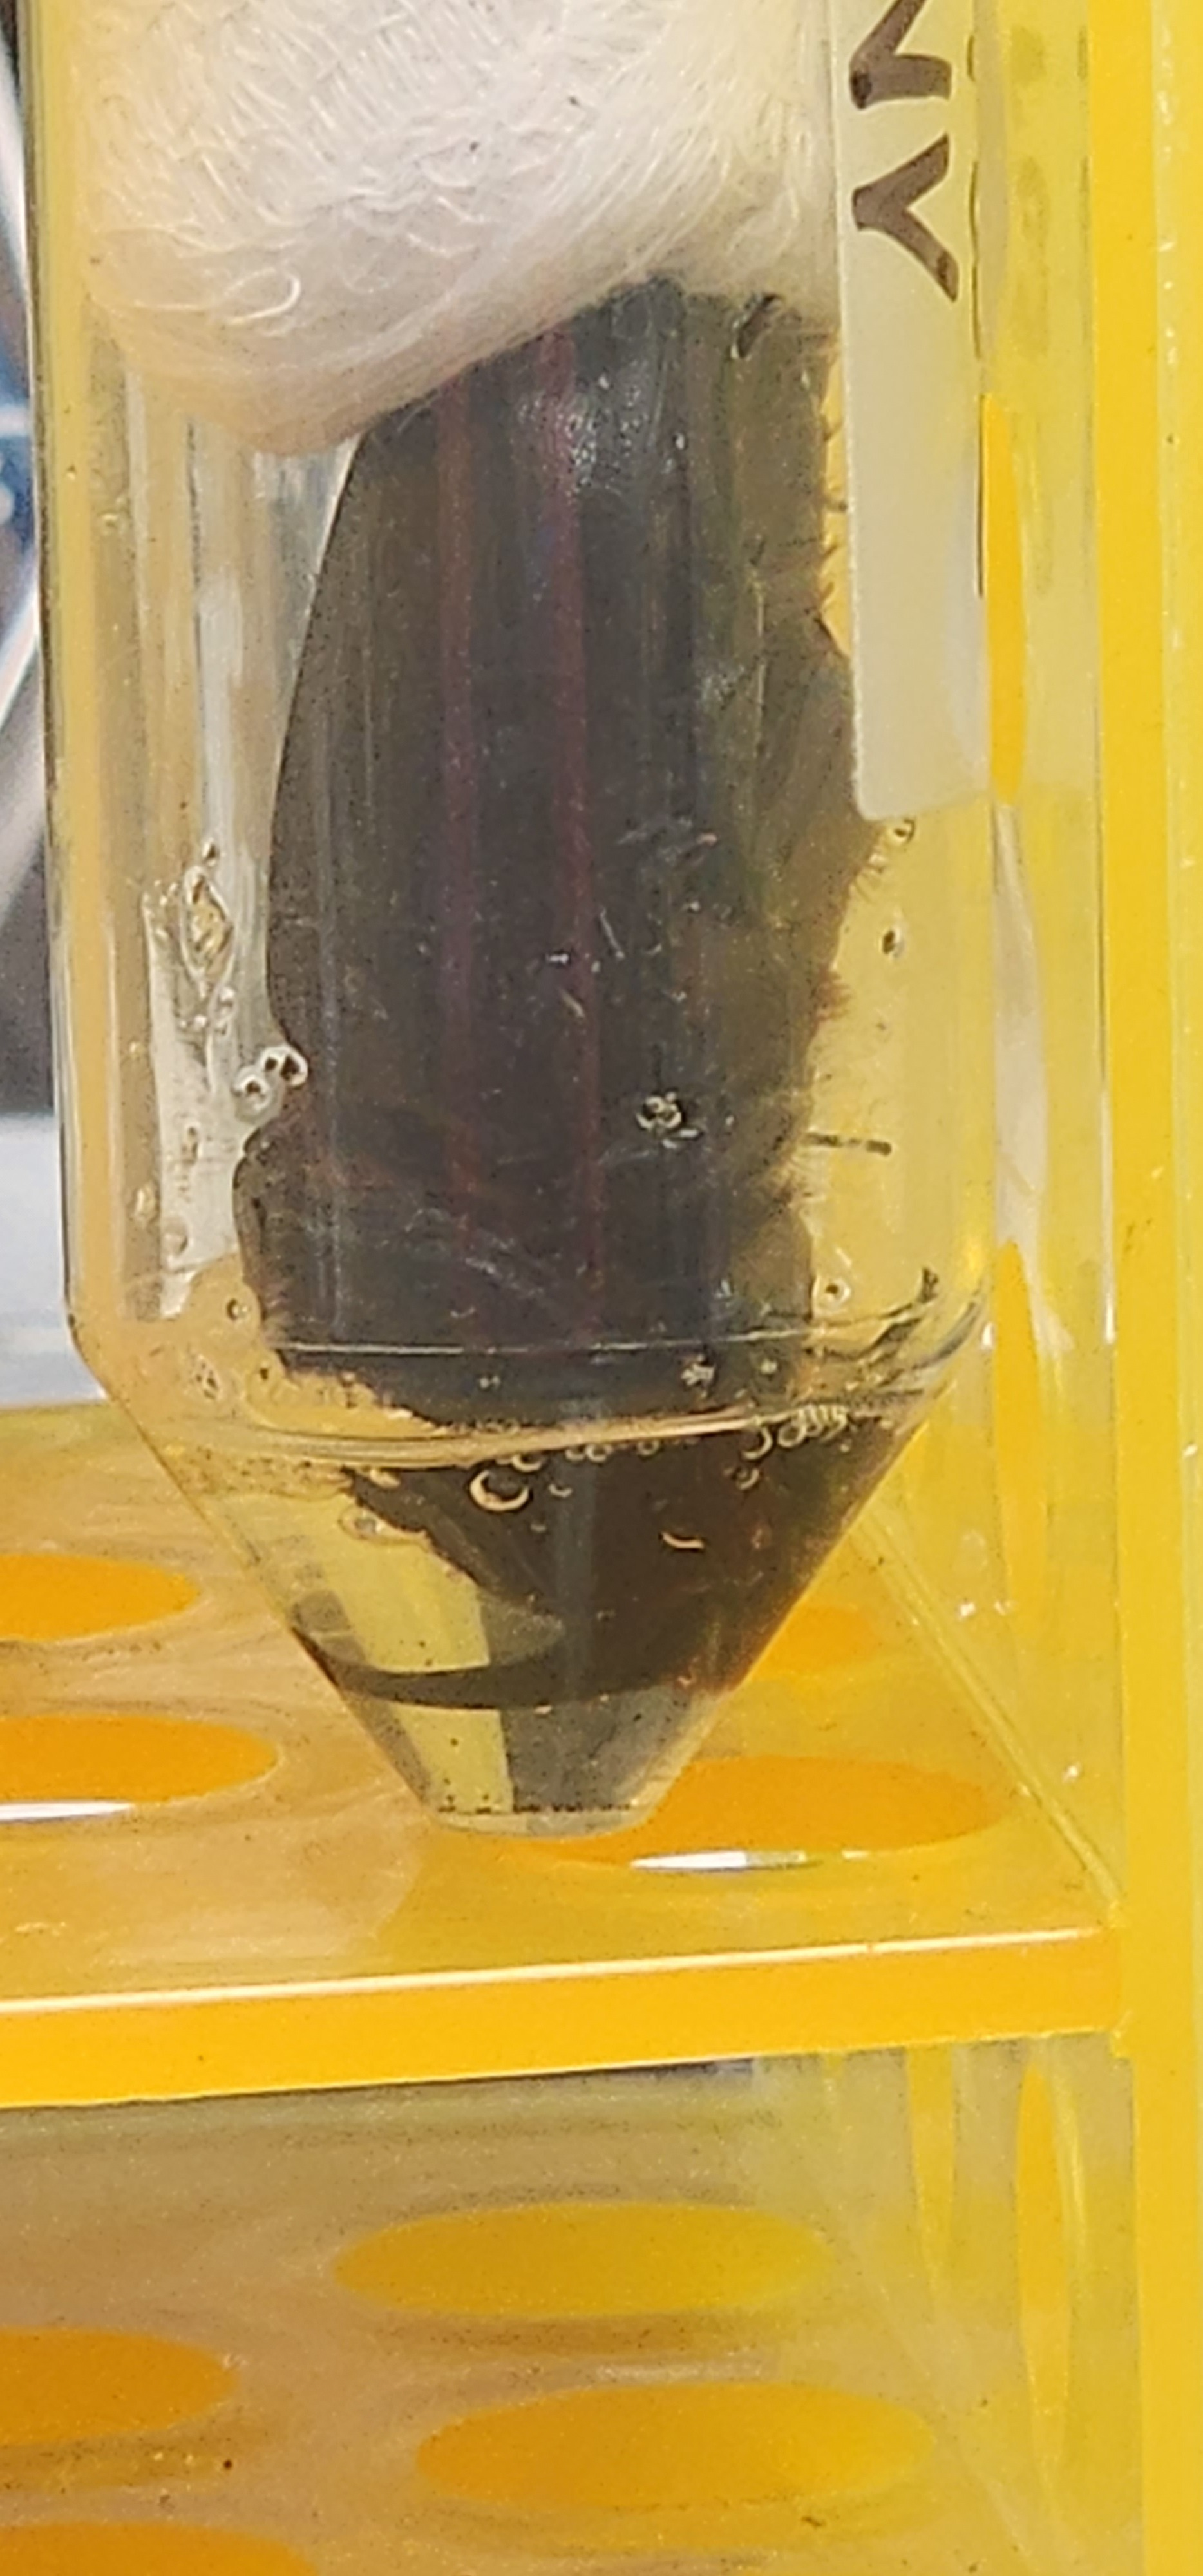
\includegraphics[width=0.5\linewidth]{images/crb-in-tube}
	\caption{CRB adult being dosed in a centrifuge tube. Mouthparts are submerged in 2 ml of 5\% sucrose solution containing 10\textsuperscript{6} infectious units of OrNV for 15 minutes. A wad of cheese cloth above the beetle keeps it in place.}
	\label{fig:crb-in-tube}
\end{figure}

\begin{figure}[H]
	\centering
	\begin{subfigure}{.5\textwidth}
		\centering
		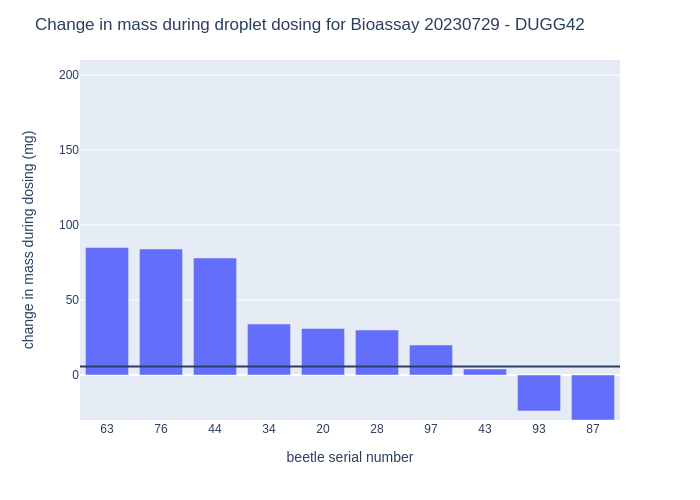
\includegraphics[width=\linewidth]{images/bioassay1}
		\caption{Droplet dosing method}
		\label{fig:sub1}
	\end{subfigure}%
	\begin{subfigure}{.5\textwidth}
		\centering
		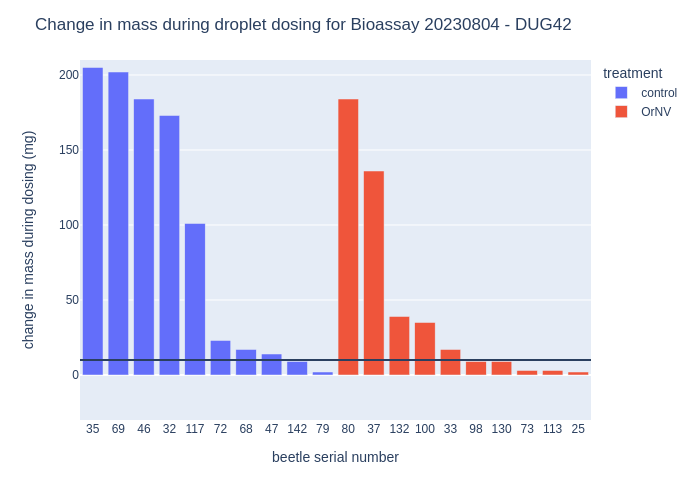
\includegraphics[width=\linewidth]{images/bioassay2}
		\caption{Tube dosing method}
		\label{fig:sub2}
	\end{subfigure}
	\caption{Black horizontal lines indicate mass containing 5,000 infective units (UI) of OrNV. This level is the the minimum dose recommended to establish infection in a susceptible beetle \parencite{AgResearch2023}.}
	\label{fig:paired-plots}
\end{figure}


\section{Notes}

\begin{enumerate}
	\item Our technique might work better if we increase sugar content (currently 5\%). Sugar content of coconut sap is 12.92\% (6.91\% sucrose, 3.48\% fructose, and 2.53\% glucose) (\cite{asgharCoconutCocosNucifera2019}).	
\end{enumerate}


\printbibliography

\end{document}
